%	This is documentation.tex, the source file of the class'
%	documentation.

%	Most of the (hopefully all) implementations of the features of
%	tufte-style-article can be seen here, as a usage example.

%	The compiled result is documentation.pdf.
%	It can be compiled as a test to see if everything works
%		--use pdflatex --shell-escape documentation.tex


\documentclass[
	a4paper,
	raggedright,
	twoside,
	12pt,
	colorful,
]{tufte-style-article}

\usepackage{lipsum}	% for blind texts generation
\usepackage{hologo}	% for special logos such as MiKTeX
\usepackage{xurl}	% to make urls break lines
\setcounter{secnumdepth}{1}

\title{The \texttt{tufte-style-article} class}
\author{Sylvain Kern}

\begin{document}

\maketitle

\vskip -25pt
\noindent\hspace{.1\textwidth}\url{https://github.com/sylvain-kern/tufte-style-article}
\vskip 25pt

\noindent
\texttt{tufte-style-article}\sidetext{Edward Tufte is a statistician, computer scientist and professor at Yale University. His personal website: \url{www.edwardtufte.com}} is a \LaTeX{} class with a design similar to Edward Tufte's works. His designs are known for their simplicty, legibleness, extensive use of sidenotes in a wide dedicated margin and tight text and graphic integration. This class is however not a rigourous copy of E.Tufte's works, it is more of an inspiration. It also includes design features from \textit{The Elements of Typographic Style}.\sidenote{\textls{\scshape robert bringhurst}, \textit{The Elements of Typographic Style}, 1999.}

This documentation gives a glimpse of what the class looks like and does, while explaining how to install and use it. I tried to make it as exhaustive as I could; some parts can however still be unexplained or so do not hesitate to ask me if something remains unclear. I tested it on several \LaTeX{} distributions, but it can still spit unexpected errors. Feel free to ask me for information or report a malfunction if you encounter one!\sidetext{See section \ref{sec:known-issues} for known issues, questions about this class and bug reporting.}

I am aware that numerous Tufte or Bringhurst-based classes exist within the \LaTeX{} nerds community, I just wanted to create my own to really dig in this design grammar. Eventually, this is just my take on what I find well-presented and eye-pleasing in a document. Everybody can feel free to adapt, customize, or contribute to this class\sidetext{I give some information for contributors on section \ref{sec:contribute}.}.

Before I dive into the details, I want to thank the members of\\\noindent \href{www.tex.stackexchange.com}{\texttt{tex.stackexchange.com}}, who are basically an endless source of knowledge. They basically prevented me from give up upon the first issue.

\newpage
\tableofcontents
\newpage


\section{Installation}

This class' source file is \texttt{tufte-style-article.cls}, available on the following repository:

\url{www.github.com/sylvain-kern/tufte-style-article}.

The file can just be put in the same folder as your main \texttt{.tex} file. Overleaf users will have to do this, since it does not support custom class installation. For Windows or Linux users with an installed \LaTeX{} distribution, please see respectively the two following sections, on how to install \texttt{tufte-style-article} on your system.

In order to make the code environments\sidenote{See section \ref{sub:code}.} and syntax highlighting work, it is needed to have Python\sidenote{Python has to be on the \texttt{PATH}.} installed on your system, along with the \texttt{pygments} package. With \texttt{pip} simply execute
\begin{codebox}{text}
pip install pygments
\end{codebox}

\subsection{\hologo{MiKTeX} users on Windows}

\begin{enumerate}

\item Create a \texttt{localtexmf}\sidenote{More on \texttt{texmf} and how to install custom classes and packages on \hologo{MiKTeX} here:\\\url{https://tex.stackexchange.com/questions/10498/installing-a-class}.} directory if you do not already have one, for instance
\begin{codebox}{text}
C:\Users\<you>\localtexmf
\end{codebox}

\item Create a \inlinecode{text}{tex\latex\} directory in the \texttt{localtexmf} one, and inside it, create a folder named \inlinecode{latex}{tufte-style-article}.

\item Paste the \inlinecode{text}{tufte-style-article.cls} file in that \inlinecode{text}{tufte-style-article} folder and you should be good. Eventually, the class file is located at
\begin{codebox}{text}
C:\Users\<you>\localtexmf\tex\latex\tufte-style-article\tufte-style-article.cls
\end{codebox}

\item Open \hologo{MiKTeX} console, go to \inlinecode{text}{Settings}, \inlinecode{latex}{Directories} tab. Click on \inlinecode{text}{add}, and enter yout \texttt{texmf} path.
\begin{codebox}{text}
C:\Users\<you>\localtexmf
\end{codebox}

\item Finally, go to the \inlinecode{text}{tasks} tab, and hit \inlinecode{text}{Refresh file name database}.

\end{enumerate}

\texttt{tufte-style-article} is now installed on your system ! \hologo{MiKTeX} will recognize and find the class file without it having to be in your project folder.

\newpage
\subsection{\TeX{} Live users on Linux}

\begin{enumerate}

\item Create a \texttt{localtexmf}\sidenote{More on \texttt{texmf} and how to install custom classes and packages on \TeX{} Live here:\\\url{https://tex.stackexchange.com/questions/96976/install-custom-cls-using-tex-live-in-local-directory}.} directory if you do not already have one, for instance
\begin{codebox}{bash}
$HOME/.texmf
\end{codebox}

\iffalse $ \fi % to keep syntax coloring neat

\item Create a \inlinecode{text}{tex/latex/} directory in the \texttt{.texmf} one, and inside it, create a folder named \inlinecode{latex}{tufte-style-article}.

\item Paste the \inlinecode{text}{tufte-style-article.cls} file in that \inlinecode{text}{tufte-style-article} folder and you should be good. Eventually, the class file is located at:
\begin{codebox}{bash}
$HOME/.texmf/tex/latex/tufte-style-article/tufte-style-article.cls
\end{codebox}

\item Update the \texttt{texmf} with
\begin{codebox}{bash}
mktexlsr $HOME/.texmf
\end{codebox}

\item Check if it worked with
\begin{codebox}{bash}
kpsewhich tufte-style-article.cls
\end{codebox}

\end{enumerate}

\texttt{tufte-style-article} is now installed on your system ! \TeX{} Live will recognize and find the class file without it having to be in your project folder.


\section{Presentation and Usage}

This section has come quite thick, so a cheat sheet should come soon to summarize all this.

\subsection{Class definition and options}

This class is named \texttt{tufte-style-article}. The preamble is therfore written as follows.

\begin{codebox}{latex}
\documentclass[<options>]{tufte-style-article}
\end{codebox}
It is inherited from the \texttt{article} class, so all the options of the latter fit in \texttt{tufte-style-article}'s options. There are also new ones for this class, which are:

\medskip
\begin{minipagewithmarginpars}[t]{.2\textwidth}
	\raggedleft
	\inlinecode{latex}{raggedright}
\end{minipagewithmarginpars}\hfill%
\begin{minipagewithmarginpars}[t]{.72\textwidth}
	Makes all paragraphs align on the left without right-justification, as it is the case in this very document.\sidetext{E.Tufte prefers left over full justification because it reduces the variation of spaces between words. The irregularities on the right makes the lines also easier to follow. Howewer, R.Bringhurst fully justifies the main text in his \textit{Elements}, so I decided to give this choice to the user. Both indent paragraphs on the first line, except just after title headers.} \\
\end{minipagewithmarginpars}
\smallskip
\begin{minipagewithmarginpars}[t]{.2\textwidth}
	\raggedleft
	\inlinecode{latex}{parskip}
\end{minipagewithmarginpars}\hfill%
\begin{minipagewithmarginpars}[t]{.72\textwidth}
	Separates paragraphs with a vertical space instead of indenting so that all text is rigorously left-aligned.
\end{minipagewithmarginpars}
\smallskip
\begin{minipagewithmarginpars}[t]{.2\textwidth}
	\raggedleft
	\inlinecode{latex}{noheaders}
\end{minipagewithmarginpars}\hfill%
\begin{minipagewithmarginpars}[t]{.72\textwidth}
	Deletes the current section reminder on page header, just displays the page number on the top outer corner.
\end{minipagewithmarginpars}
\smallskip
\begin{minipagewithmarginpars}[t]{.2\textwidth}
	\raggedleft
	\inlinecode{latex}{casual}
\end{minipagewithmarginpars}\hfill%
\begin{minipagewithmarginpars}[t]{.72\textwidth}
	Makes all sections numberless. Puts them natively in the toc anyway.
\end{minipagewithmarginpars}
\smallskip
\begin{minipagewithmarginpars}[t]{.2\textwidth}
	\raggedleft
	\inlinecode{latex}{sans}
\end{minipagewithmarginpars}\hfill%
\begin{minipagewithmarginpars}[t]{.72\textwidth}
	Turns the font to sans serif Source Sans Pro, for extreme casualness.
\end{minipagewithmarginpars}
\smallskip
\begin{minipagewithmarginpars}[t]{.2\textwidth}
	\raggedleft
	\inlinecode{latex}{colorful}
\end{minipagewithmarginpars}\hfill%
\begin{minipagewithmarginpars}[t]{.72\textwidth}
	Like in this document, makes titles, figure labels and note numbers colored. The accent color is defined by \texttt{main\_accent}.
\end{minipagewithmarginpars}
\smallskip
\begin{minipagewithmarginpars}[t]{.2\textwidth}
	\raggedleft
	\inlinecode{latex}{notufte}
\end{minipagewithmarginpars}\hfill%
\begin{minipagewithmarginpars}[t]{.72\textwidth}
	Remove margins. Turns sidenotes to footnotes and makes figure captions appear under them. Appropried for small casual reports or for \texttt{pandoc conversion}.
\end{minipagewithmarginpars}


\subsection{The big margin}

As one may have noticed, there is a big outer margin, a design feature present in all E.Tufte's works but also in the \textit{Elements of Typographic style}. I find this design --a \textit{1.5-column} setup-- to have many advantages over a regular one-column setup. Here are a few reasons why.
\begin{itemize}\tightlist
	\item The main text block has a reduced width of about thirteen words per line, which makes the eyes follow the lines easier.

	\item The layout is less constrained thanks to the negative space freed in the margin.

	\item The margin can be used to place elements that would break the main prose, such as sidenotes,\sidenote{Hello there!} captions of figures, tables and other stuff, and even small figures. This tidies up the main text area while making margin stuff immediately noticeable, but not disturbing.

	\item The overall text-image inclusion comes tighter and more natural.
\end{itemize}
All in all, this design is neither too crowded as everything is at its place, nor too empty due to huge blank margins.

To insert a numbered margin note, use \inlinecode{latex}{\sidenote{<your note>}}. This gives the following result in the margin.\sidenote{This is a numbered note.}

To insert an unnumbered piece of text in the margin, use\\\noindent\inlinecode{latex}{\sidetext{<your text>}}, which gives the following result in the margin.\sidetext{This is unnumbered margin text.}

All pieces of text in the margin are in \texttt{\textbackslash footnotesize} and \texttt{\textbackslash raggedright}, as defined in this class' macros.

To insert raw, unformatted text or graphics or whatever in the margin, use the command\\ \inlinecode{latex}{\marginpar{<unformatted margin text>}} and it will look like what appears here in the margin\marginpar{This is just unformatted text in the margin. It is in \texttt{\textbackslash normalsize}, which makes it stick out way too much.}. Note how it is the same size as the main text. Also \LaTeX{} tries to fully justifiy it which is hard on such a small width.


\subsection{Paragraphs}

The main text is structured in paragraphs. They can be left-aligned as it is the case here, or fully justified according to your taste, depending on the given class options. Likewise, the paragraphs are whether indented or separated with a vertical space.

The indents are one em wide, \textit{i.e.} the size of the font in pt. If you choose a 11 pt size in the options declaration of the class, then the indent will be 11 pt wide.

\begingroup
\setlength{\parindent}{0em}
\setlength{\parskip}{1em}
This one and the following are paragraphs with vertical space separation. It works better for documents not intended to be read linearly, or when there is few text compared to figures, equations or anything which does not fit in the prose.

The vertical space looks like this, with a separation of one em. This is just some more text to fill the paragraph, and give a glimpse of the overall look. Quick reminder, load the vertical separation with the \inlinecode{latex}{parskip} option in the class definition.
\endgroup

\begin{wide}
\hspace{1em}
There is a way to make paragraphs stretch all the way to the margins, like this one.	See how it continues and reaches for the most outer or inner margin. It also works for two-sided documents so that for odd pages it stretches to the right, and for even pages it stretched to the left. Of course, side notes might be difficult to use here, and I do not predict how \inlinecode{latex}{\sidenote} and  \inlinecode{latex}{\sidetext} act here, but it may become handy to have an environment stretch a bit more than the regular text span.

To stretch the main text area to the margins, use the following environment.
\begin{codebox}{latex}
\begin{wide}
<...your content will be displayed in a wide mode...>
\end{wide}
\end{codebox}

\LaTeX{} may not get the formatting right upon first compilation, so if that occurs, just re-execute the compiling program and it should work properly.
\end{wide}


\subsection{Fonts}

The main serif font is Linux Libertine,\sidetext{Although E.Tufte uses \href{www.catalog.monotype.com/family/monotype/bembo}{Monotype Bembo} as his main serif font, Libertine seems to be a fair alternative, from the same family, and easy to get with \LaTeX{}.} loaded with the \href{www.ctan.org/pkg/libertinus}{\texttt{libertinus}} package. I find it really legible and well-balanced, while being less harsh than Computer Modern, the default \LaTeX{} font. \href{www.ctan.org/pkg/libertinus}{\texttt{libertinus}} has full math support too with \href{www.ctan.org/pkg/libertinust1math}{\texttt{libertinust1math}}; here are some examples:
$$
e^x = \sum_{n=0}^{+\infty} \frac{x^n}{n!} \;;
$$

$$
\frac{{\hat{\vec p}}^2}{2m}\ket{\Psi(t)} + V\left(\hat{\vec r},t\right)\ket{\Psi(t)} = i\hbar \pdv{}{t}\ket{\Psi(t)} \;;
$$

$$
x_\pm = \frac{-b \pm \sqrt{b^2 - 4ac}}{2a}\;;
$$

$$
\int_{-\infty}^{+\infty} e^{-\alpha x^2} \dd{x} = \sqrt\frac{\pi}{\alpha}.
$$

\begin{equation}
\psi(\vec r) = \frac{j}{\lambda} \iint_S \psi(\vec{r_0})\frac{e^{jk|\vec r - \vec r_0|}}{|\vec r - \vec r_0|}\dd S.
\end{equation}

\begingroup\sffamily
The sans-serif font is Gillius from the \href{www.ctan.org/pkg/gillius}{\texttt{gillius}} package, which is almost identical as Gill Sans, E.Tufte's choice for sans-serif and book titling. It does not clash with Libertine while being elegant and readable. It particularly suits for titles or page headers as it can be seen on this document.
\endgroup

\begingroup\ttfamily
The mono font is Droid Sans Mono, from the \href{www.ctan.org/pkg/droid}{\texttt{droidmono}} package. It has a more of a sans-serif style unlike \href{www.ctan.org/tex-archive/fonts/psfonts/psnfss-source/courier}{Courier} or \href{www.ctan.org/tex-archive/fonts/cm/}{Computer Modern Teletype}, \LaTeX{}'s default mono font. I find it lighter and more adapted for code snippets\sidetext{For examples of code writing with this class, see section \textcolor{lighter_accent}{code}.}. The typographic gray is also about the same as Libertine, so that little urls, emails or code references typed with Droid Sans will not stick out in the serif text\sidenote{If you want inline pieces of code to stick out, don't worry, macros are provided. See section \ref{sub:code}.}.
\endgroup


\subsection{Figures, tables and floating stuff}

\subsubsection{Figure integration}

Edward Tufte's designs are known to be really tight when it comes to including images with text. The main pet peeve I had with one-column designs is when I included a small figure in the document, it had to visually break the text and generate large unpleasing blank spaces. Also, more often than not, the text width was too much for the images, resulting in huge one-liner captions for very small figures.

The 1.5-column design fixes this by putting all captions in the margins, as well as small enough figures, which tidies the document a lot.

\textfig[1]{figures/bretagne.png}{1919 map of the Finistère in French Brittany. This figure is in the main text column, with a caption in the margin aligned with the top of the image. For images narrower than the text width, they will be outer-aligned so that they remain just next their caption.}{fig:figure-text}

% \begin{figure}[htbp]
% 	\sidecaption{1919 map of the Finistère in French Brittany. This figure is in the main text column, with a caption in the margin aligned with the top of the image. For images with width less than the text width, they will be outer-aligned so that they are close to the caption.}\label{fig:figure-text}
% 	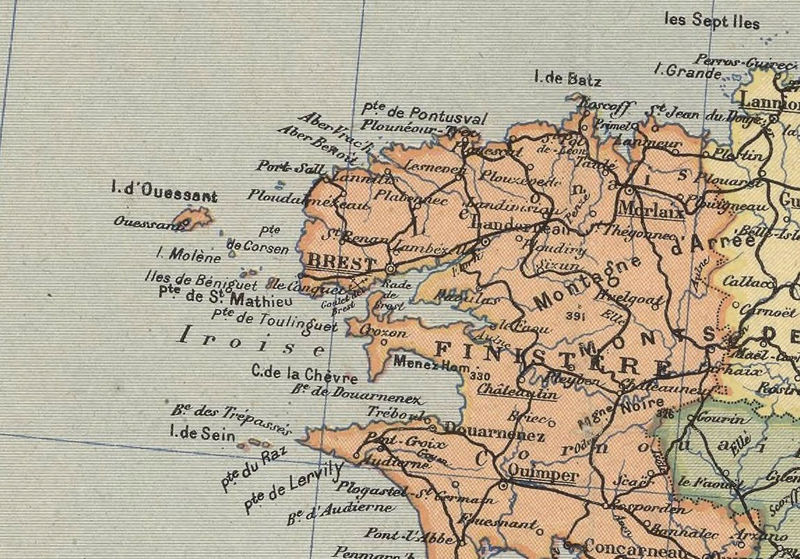
\includegraphics[width = \linewidth, outer]{figures/bretagne.png}
% \end{figure}


To put a graphics in the text like in the figure \ref{fig:figure-text}, use\sidenote{The \texttt{\textbackslash label} \textit{has} to be inside the \texttt{\textbackslash sidecaption} command, otherwise references with \texttt{\textbackslash ref} won't work.}

\begin{codebox}{latex}
\begin{figure}
	\sidecaption{<caption>\label{<label>}} % put this on top
	% \label HAS to be inside the \sidecaption
	\includegraphics[]{<>} % or tikz or anything
\end{figure}
\end{codebox}

\marginfig{figures/marine-knots.jpg}{The most common sea boat knots. This image can be displayed rather small, so it fits in the margin. The caption is displayed below.}{fig:figure-margin}

To put a figure in the margin like the figure \ref{fig:figure-margin}, use

\begin{codebox}{latex}
	\begin{marginfigure}
		\includegraphics[]{<>} % or tikz or anything
		\caption{<caption>\label{<label>}}
	\end{figure}
\end{codebox}

For wide figures like the figure \ref{fig:figure-fullwidth}, use

\begin{codebox}{latex}
	\begin{figure*}
		\includegraphics[]{<>} % or tikz or anything
		\sidecaption{<caption>\label{<label>}}
	\end{figure*}
\end{codebox}


\widefig{figures/usa-census.png}{The US census map from data collected in 2010 -- \url{www.ecpmlangues.u-strasbg.fr}\\This is a wide figure, stretching from the innermost to the outermost margin.}{fig:figure-fullwidth}


\subsubsection{Shortcuts}

I find typing figure environments repetitive for long (even short) documents, so I made the following macro for figures with \texttt{\textbackslash sidecaption}s :

\begin{codebox}{latex}
\textfig[<optional width>]{<file path>}{<caption>}{<label>}
\end{codebox}

The \inlinecode{text}{<optional width>} is a number between zero and one wich determines the image width relative to the text width. The default value is 1, like on the figure \ref{fig:figure-text}.

The same macros are provided for images in the magins and wide images, respectively shown in figures \ref{fig:figure-margin} and \ref{fig:figure-fullwidth}

\begin{codebox}{latex}
% figure in the margin
\marginfig[<optional width>]{<file path>}{<caption>}{<label>}
% wide figure
\widefig[<optional width>]{<file path>}{<caption>}{<label>}
\end{codebox}



If for any reason a figure caption has to be put in the main text block, no worries, just use the regular \texttt{figure} environment. The following shortcut macros will also do. The result of \inlinecode{latex}{\plainfig} is shown in figure \ref{fig:figure-plain}.

\begin{codebox}{latex}
% plain figure with textwidth
\plainfig[<optional width>]{<file path>}{<caption>}{<label>}
% plain figure with full width
\plainwidefig[<optional width>]{<file path>}{<caption>}{<label>}
\end{codebox}


\plainfig[.7]{figures/mandelbrot.png}{The Mandelbrot set with different depths of iteration. This caption is not in the margin but in the main text area. It can sometimes be useful, for example with really really long captions.}{fig:figure-plain}

\newpage

\subsubsection{Tables (in progress\dots)}

This is still in development, table coverage will be provided soon ! (it will be all like figures)


\iffalse
\begin{texttable}{Table inserted in text}{tab:texttable}
\begin{tabularx}{\textwidth}{lll}
\multicolumn{4}{l}{\bfseries The Vox-ATypI classification}\\
\toprule
Classical & Modern & Calligraphics \\
yo & yo & yo \\
yo & yo & yo \\
yo & yo & yo \\
\bottomrule
\end{tabularx}
\end{texttable}
\fi


\subsection{Code}
\label{sub:code}

Code can be inserted, whether with simple code boxes or captioned snippets that look like the following.
\begin{snippet}{c}{Hello world in C. This is a captioned code snippet.}{snp:hello-world}
int main(int argc, char *argv[]) {
	printf("Hello world!");
	return 0;
}
\end{snippet}

The background is a light gray that helps make the code stick out just enough without distracting the eye too much. The code itself is syntax colored according to the used language. There are several environments for code boxes, explained below.

\newpage

For a simple code box with neither line numbering nor caption, the macro environment is the following.

\sidetext{%
This supports most of the classic languages. Here are some examples for the language option:

\inlinecode{text}{c},

\indent\inlinecode{text}{c++},

\indent\inlinecode{text}{python},

\indent\inlinecode{text}{java},

\indent\inlinecode{text}{latex}\dots

If a specific language is not recognized, use the \inlinecode{text}{text} option instead: it will display the code without syntax coloring.
}%
\begin{altcodebox}{latex}
\begin{codebox}{<your language in lowercase>}
<
Your code. It can contain all special characters such as { } ( ) [ ] \ % (the percent mark here is grayed just because on this very code box the language is set on latex)
It break lines.
It will end only when reading the %\end{codebox} below.
>
\end{codebox}
\end{altcodebox}

For a code box \textit{with} line numbering --still without a caption-- use the following environment.
\begin{altcodebox}{latex}
\begin{codeboxnum}{<your language in lowercase>}
<your code>
\end{codeboxnum}
\end{altcodebox}

For captioned code snippets, the same environments exist, as shown as follows. For example, the listings \ref{snp:hello-world} and \ref{snp:snowflakeos} are respectively unnumbered and numbered code snippets.

\begin{codebox}{latex}
\begin{snippet}{<language>}{<caption>}{<label>}
This code will be displayed in a captioned code box, without line numbering.
\end{snippet}

\begin{snippetnum}{<language>}{<caption>}{<label>}
This code will be displayed in a captioned code box, with line numbering.
\end{snippetnum}
\end{codebox}

Small pieces of code can be useful to put in flow of the text. This class provides a command to things like this: \inlinecode{c++}_public int size() {}_. Use the following to insert a piece of code in the text.


\sidetext{If the piece of code inside the \inlinecode{latex}{\inlinecode} contains curly braces, use another character to delimit your code, the same at beginning and end. Underscore (\texttt{\char`_}) and pipe (\texttt{|}) will do fine.}
\begin{codebox}{latex}
\inlinecode{<language>}{<your code>}
% if there are curly braces in your code
\inlinecode{<language>}_<your code>_ % or
\inlinecode{<language>}|<your code>|
\end{codebox}

\inlinecode{latex}{\inlinecode} does not break at lines, so be careful, it can sometimes protrude on the right margin. If it is the case, go to a new line by inserting \inlinecode{latex}{\\} just before \inlinecode{latex}{\inlinecode}.


The following chunk is an example snippet to show the look when the code is a bit heftier. See how the box breaks at the end of the page.

\begin{snippetnum}{c}{A source code snippet of \texttt{29jm}'s stunningly amazing \href{https://github.com/29jm/SnowflakeOS}{\texttt{SnowflakeOS}}. This is a numbered code snippet that goes through several pages.}{snp:snowflakeos}
#include <kernel/multiboot2.h>
#include <kernel/sys.h>

static const char* tag_table[] = {
	"TAG_END",
	"TAG_CMDLINE",
	"<unknown>",
	"TAG_MODULE",
	"TAG_MEM",
	"TAG_BOOTDEV",
	"TAG_MEMMAP",
	"TAG_VBE",
	"TAG_FB",
	"<unknown>",
	"TAG_APM",
	"<unknown>",
	"<unknown>",
	"<unknown>",
	"TAG_RSDP1",
	"TAG_RSDP2",
};

/* Prints the multiboot2 tags given by the bootloader.
*/
void mb2_print_tags(mb2_t* boot) {
	if (boot->total_size <= sizeof(mb2_t)) {
		printke("no tags given");
		return;
	}

	mb2_tag_t* tag = boot->tags;
	mb2_tag_t* prev_tag = tag;

	do {
		const char* tag_name;

		if (tag->type < sizeof(tag_table) / sizeof(tag_table[0])) {
			tag_name = tag_table[tag->type];
		} else {
			tag_name = "<unknown>";
		}

		printk("%12s (%2d): %d bytes", tag_name, tag->type, tag->size);

		prev_tag = tag;
		tag = (mb2_tag_t*) ((uintptr_t) tag + align_to(tag->size, 8));
	} while (prev_tag->type != MB2_TAG_END);
}

/* Returns the first multiboot2 tag of the requested type.
*/
mb2_tag_t* mb2_find_tag(mb2_t* boot, uint32_t tag_type) {
	mb2_tag_t* tag = boot->tags;
	mb2_tag_t* prev_tag = tag;

	do {
		if (tag->type == tag_type) {
			return tag;
		}

		prev_tag = tag;
		tag = (mb2_tag_t*) ((uintptr_t) tag + align_to(tag->size, 8));
	} while (prev_tag->type != MB2_TAG_END);

	return NULL;
}
\end{snippetnum}


\subsection{Compilation}

This class compiles with \texttt{pdflatex}. I tested it with \hologo{MiKTeX} on Windows, \TeX-live on Linux and Overleaf. If you use code boxes or snippets, make sure you compile with the \texttt{--shell-escape} flag. Eventually, the following compilation line should work everywhere.
\begin{codebox}{text}
pdflatex --shell-escape yourdocument.tex
\end{codebox}
The compilation times can be quite long, especially if there is a lot of heavy code,\sidetext{I am still working to optimize the class by reducing the compilation time.} hopefully it is not a problem for most cases.


\section{Customization possibilities}
\label{sec:customization-possibilities}

\subsection{Language}

\texttt{babel} works fine, but it can sometimes change some design and layout features.\sidenote{For example, the \inlinecode{text}{french} option changes bullet lists for dashes, indents paragraphs just after section headers, and puts figure labels to \inlinecode{text}_\textsc{}_.} To prevent \texttt{babel} from changing anything, use the following in the preamble --here it is shown for french, you can adapt the language.
\begin{codebox}{latex}
\frenchsetup{StandardLayout=true, SmallCapsFigTabCaptions=false}
\end{codebox}


\section{Contribute}
\label{sec:contribute}

I am always open to improvements, so feel free to fork the repository to make this the way you want it to be. I am relatively new to \LaTeX{}, so I am eager to put the class to higher standards.


\section{Known issues}
\label{sec:known-issues}

In this section I gather the issues that have popped and been reported. I will try to fix them as best as I can. If you spot a malfunction of any kind in this class or you just have a question about all this, feel free to raise an issue on GitHub or send me an email at:

\href{mailto:sylvain.kern98@gmail.com}{\texttt{sylvain.kern98@gmail.com}}.

\bigskip

\begin{itemize}\tightlist
\item When used, \inlinecode{text}{colorful}, \inlinecode{text}{sans}, and \inlinecode{text}{notufte} are considered unused. It generates the following warning :
\begin{codebox}{text}
Unused global option(s) : colorful.
\end{codebox}
\item Bad page breaks can still occur for \inlinecode{latex}_\textfig{}_, \inlinecode{latex}_\widefig{}_, and code snippet environments.
\item Marginpar systematically generates the following warnings:
\begin{codebox}{text}
Marginpar on page 1 moved.
\end{codebox}
\item I have to work on overfull \textbackslash hboxes.
\item Need to renew the \texttt{itemize} and \texttt{enumerate} environment to \texttt{\textbackslash tightlist} them up.
\end{itemize}


\section{Package definition}

The class requires the following packages :
\begin{codebox}{latex}
%	P A C K A G E   D E F I N I T I O N
%
\RequirePackage{geometry}		% page geometry, margin definition
\RequirePackage{emptypage}		% if a page is empty, is is really empty
\RequirePackage{fullwidth}		% for wide environments
\RequirePackage{sidenotes}		% for margin stuff
\RequirePackage[
	hypcap=false				% hypcap=true spits an error
]{caption}						% for caption formatting
\RequirePackage[T1]{fontenc}	% font encoding
\RequirePackage[osf]{libertinus}% main font
\RequirePackage{libertinust1math}
\RequirePackage{gillius}		% sans font
\if@sans
	\RequirePackage[			% font for full sans document
		osf,
		default
	]{sourcesanspro}
\fi
\RequirePackage[
	defaultmono,
	scale=.86
]{droidsansmono}				% mono font
\RequirePackage{ragged2e}		% for better raggedright
\RequirePackage{titlesec}		% header customization
\RequirePackage{titletoc}		% toc customization
\RequirePackage{fancyhdr}		% page header customization
\RequirePackage{graphicx}		% for images
\RequirePackage[
	protrusion=true,
	expansion=true,
	final,
	tracking,
]{microtype}					% microtypography: fine-tuning in text
\RequirePackage{amsfonts}		% math fonts
\RequirePackage{amsmath}		% math stuff
\RequirePackage{mathtools}		% amsmath extension
\RequirePackage{physics}		% handy shortcuts for physics
\RequirePackage{minted} 		% for code display
\RequirePackage{xcolor}			% colorz
\RequirePackage[framemethod=TikZ]{mdframed} % for custom code boxes
\RequirePackage{tabularx}		% adaptive columns on tables
\RequirePackage{booktabs}		% better looking tables
\RequirePackage{enumitem}		% better looking lists
\RequirePackage[
	super,
	square
]{natbib}						% customize \cite{}
\RequirePackage[hidelinks]{hyperref}	% automatic references in pdf
\RequirePackage{etoolbox}		% really idk what this does
\RequirePackage{verbatim}   	% for verbatim environments
\end{codebox}


\end{document}